\chapter{Evaluation}
\label{chap:evaluation}

\indent \indent
This chapter evaluates the project's implementation using three main criteria: the extent to which it meets the success criteria detailed in §\ref{sec:requirements},  the applicability of HE to inference algorithms, and its practicality regarding current, real-world surveillance technology. Consequently, the chapter is divided into three sections to tackle each criterion distinctly. Both quantitative and qualitative analysis is used throughout the chapter to analyse the implementation's performance and make predictions about the scope to which the investigation may be extended in future. Unless otherwise specified, the data presented was generated using $32 \times 32$ pixel images from the Moving-MNIST dataset.

\section{Requirements Analysis}
\begin{table}[h!]
    \centering
    \def\arraystretch{1.25}
    \begin{tabular}{|c|c|p{9.6cm}|}
        \hline
        \textrm{\textbf{Requirement}} & \textrm{\textbf{Achieved?}} & \textrm{\textbf{Justification}} \\
        \hline \hline
        \texttt{A1} & \cmark & \textrm{The project contains a client-server application that allows videos to be homomorphically encrypted and transmitted across a network, with implementation techniques detailed in §\ref{sec:networking}.} \\
        \hline
        \texttt{A2} & \cmark & \textrm{The project contains several algorithms that are able to extract moving objects from homomorphically encrypted videos, with implementation techniques detailed in §\ref{sec:inference}.} \\
        \hline
        \texttt{A3} & \cmark & \textrm{The accuracy of HE inference algorithms are evaluated to investigate their efficacy and applicability in §\ref{sec:integration}.} \\
        \hline \hline
        \texttt{B1} & \cmark & \textrm{The MeKKS scheme, detailed in §\ref{sec:mekks}, provides a complete implementation of the fundamental principles of the CKKS HE scheme.} \\
        \hline
        \texttt{B2} & \xmark &  \textrm{Due to time constraints, an independent investigation into the security of HE schemes could not be completed. However, only well-established, trusted schemes were considered; hence CKKS was selected and reimplemented over less secure schemes.} \\
        \hline
        \texttt{B3} & \xmark & \textrm{The implementation of moving object detection algorithms proved to be more open than expected. Consequently, more time was dedicated to further understanding this area rather than expanding into other inference paradigms.} \\
        \hline
    \end{tabular}
    \caption[Requirements Analysis]{Requirements analysis.}
    \label{tab:requirements}
\end{table}
\setlength{\leftskip}{0.25cm}
\indent \indent
The success criteria in §\ref{sec:requirements} were split into two categories: \textit{core} and \textit{extensions}.  As detailed in Table \ref{tab:requirements}, All three of the core criteria were implemented, and one of the three extensions has also been completed. The open-ended nature of this project means that defining a \textit{completed} state for some criterium was not trivial. For example, for criterium \texttt{A2}, while some algorithms have been implemented in their entirety, others require further investigation. However, it was important to have a goal for each criterium to properly plan the project and consider all aspects equally. Therefore, a justification for the state of each criterium has been included.

\setlength{\leftskip}{0cm}




\section{Homomorphic Encryption Integration}
\label{sec:integration}
\setlength{\leftskip}{0.25cm}
\indent \indent
Adapting moving object detection algorithms for the HE domain proved to be the project's biggest challenge. The limited number of operations available, combined with the limited number of applications supported by ciphertexts, means some aspects of inference cannot be recreated. Particular challenges came when trying to implement the median filter and a GMM.
\smallskip \\ \indent
However, frame differencing, the mean filter, and the Gaussian average methods of background subtraction were successfully implemented using the techniques described in §\ref{sec:adaptations}. A sample of the results from each of these algorithms running on the Moving-MNIST dataset is provided in Figure \ref{fig:mnistInferenceResults}, and an example of performance on the LASIESTA dataset is included in Appendix \ref{app:LASIESTA}.
\begin{figure}
    \centering
    \begin{subfigure}[t]{0.9\textwidth}
        \centering
        \begin{subfigure}[t]{0.19\textwidth}
            \centering
            \textrm{Frame 0} \medskip \\
            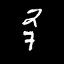
\includegraphics[scale=1]{figures/mnist0/frame0}
        \end{subfigure}
        \hfill
        \begin{subfigure}[t]{0.19\textwidth}
            \centering
            \textrm{Frame 4} \medskip \\
            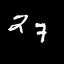
\includegraphics[scale=1]{figures/mnist0/frame4}
        \end{subfigure}
        \hfill
        \begin{subfigure}[t]{0.19\textwidth}
            \centering
            \textrm{Frame 8} \medskip \\
            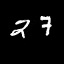
\includegraphics[scale=1]{figures/mnist0/frame8}
        \end{subfigure}
        \hfill
        \begin{subfigure}[t]{0.19\textwidth}
            \centering
            \textrm{Frame 12} \medskip \\
            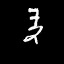
\includegraphics[scale=1]{figures/mnist0/frame12}
        \end{subfigure}
        \hfill
        \begin{subfigure}[t]{0.19\textwidth}
            \centering
            \textrm{Frame 16} \medskip \\
            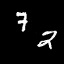
\includegraphics[scale=1]{figures/mnist0/frame16}
        \end{subfigure}
        \caption{Original Moving-MNIST frames.}
    \end{subfigure}
    \\ \bigskip
    \begin{subfigure}[t]{0.9\textwidth}
        \centering
        \begin{subfigure}[t]{0.19\textwidth}
            \centering
            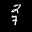
\includegraphics[scale=2]{figures/CKKS-DIFFERENCING/frame0}
        \end{subfigure}
        \hfill
        \begin{subfigure}[t]{0.19\textwidth}
            \centering
            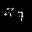
\includegraphics[scale=2]{figures/CKKS-DIFFERENCING/frame4}
        \end{subfigure}
        \hfill
        \begin{subfigure}[t]{0.19\textwidth}
            \centering
            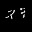
\includegraphics[scale=2]{figures/CKKS-DIFFERENCING/frame8}
        \end{subfigure}
        \hfill
        \begin{subfigure}[t]{0.19\textwidth}
            \centering
            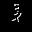
\includegraphics[scale=2]{figures/CKKS-DIFFERENCING/frame12}
        \end{subfigure}
        \hfill
        \begin{subfigure}[t]{0.19\textwidth}
            \centering
            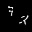
\includegraphics[scale=2]{figures/CKKS-DIFFERENCING/frame16}
        \end{subfigure}
        \caption{Frame Differencing with CKKS.}
    \end{subfigure}
    \\ \bigskip
    \begin{subfigure}[t]{0.9\textwidth}
        \centering
        \begin{subfigure}[t]{0.19\textwidth}
            \centering
            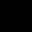
\includegraphics[scale=2]{figures/CKKS-MEAN/frame0}
        \end{subfigure}
        \hfill
        \begin{subfigure}[t]{0.19\textwidth}
            \centering
            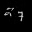
\includegraphics[scale=2]{figures/CKKS-MEAN/frame4}
        \end{subfigure}
        \hfill
        \begin{subfigure}[t]{0.19\textwidth}
            \centering
            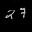
\includegraphics[scale=2]{figures/CKKS-MEAN/frame8}
        \end{subfigure}
        \hfill
        \begin{subfigure}[t]{0.19\textwidth}
            \centering
            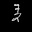
\includegraphics[scale=2]{figures/CKKS-MEAN/frame12}
        \end{subfigure}
        \hfill
        \begin{subfigure}[t]{0.19\textwidth}
            \centering
            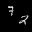
\includegraphics[scale=2]{figures/CKKS-MEAN/frame16}
        \end{subfigure}
        \caption{Mean Filter with CKKS.}
    \end{subfigure}
    \\ \bigskip
    \begin{subfigure}[t]{0.9\textwidth}
        \centering
        \begin{subfigure}[t]{0.19\textwidth}
            \centering
            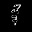
\includegraphics[scale=2]{figures/CKKS-GAUSSIAN/frame0}
        \end{subfigure}
        \hfill
        \begin{subfigure}[t]{0.19\textwidth}
            \centering
            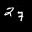
\includegraphics[scale=2]{figures/CKKS-GAUSSIAN/frame4}
        \end{subfigure}
        \hfill
        \begin{subfigure}[t]{0.19\textwidth}
            \centering
            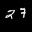
\includegraphics[scale=2]{figures/CKKS-GAUSSIAN/frame8}
        \end{subfigure}
        \hfill
        \begin{subfigure}[t]{0.19\textwidth}
            \centering
            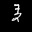
\includegraphics[scale=2]{figures/CKKS-GAUSSIAN/frame12}
        \end{subfigure}
        \hfill
        \begin{subfigure}[t]{0.19\textwidth}
            \centering
            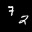
\includegraphics[scale=2]{figures/CKKS-GAUSSIAN/frame16}
        \end{subfigure}
        \caption{Gaussian Average with CKKS.}
    \end{subfigure}
    \\ \bigskip
    \begin{subfigure}[t]{0.9\textwidth}
        \centering
        \begin{subfigure}[t]{0.19\textwidth}
            \centering
            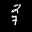
\includegraphics[scale=2]{figures/MeKKS-DIFFERENCING/frame0}
        \end{subfigure}
        \hfill
        \begin{subfigure}[t]{0.19\textwidth}
            \centering
            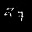
\includegraphics[scale=2]{figures/MeKKS-DIFFERENCING/frame4}
        \end{subfigure}
        \hfill
        \begin{subfigure}[t]{0.19\textwidth}
            \centering
            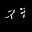
\includegraphics[scale=2]{figures/MeKKS-DIFFERENCING/frame8}
        \end{subfigure}
        \hfill
        \begin{subfigure}[t]{0.19\textwidth}
            \centering
            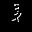
\includegraphics[scale=2]{figures/MeKKS-DIFFERENCING/frame12}
        \end{subfigure}
        \hfill
        \begin{subfigure}[t]{0.19\textwidth}
            \centering
            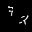
\includegraphics[scale=2]{figures/MeKKS-DIFFERENCING/frame16}
        \end{subfigure}
        \caption{Frame Differencing with MeKKS.}
    \end{subfigure}
    \\ \bigskip
    \begin{subfigure}[t]{0.9\textwidth}
        \centering
        \begin{subfigure}[t]{0.19\textwidth}
            \centering
            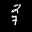
\includegraphics[scale=2]{figures/MeKKS-DIFFERENCING/frame0}
        \end{subfigure}
        \hfill
        \begin{subfigure}[t]{0.19\textwidth}
            \centering
            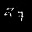
\includegraphics[scale=2]{figures/MeKKS-DIFFERENCING/frame4}
        \end{subfigure}
        \hfill
        \begin{subfigure}[t]{0.19\textwidth}
            \centering
            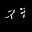
\includegraphics[scale=2]{figures/MeKKS-DIFFERENCING/frame8}
        \end{subfigure}
        \hfill
        \begin{subfigure}[t]{0.19\textwidth}
            \centering
            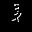
\includegraphics[scale=2]{figures/MeKKS-DIFFERENCING/frame12}
        \end{subfigure}
        \hfill
        \begin{subfigure}[t]{0.19\textwidth}
            \centering
            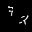
\includegraphics[scale=2]{figures/MeKKS-DIFFERENCING/frame16}
        \end{subfigure}
        \caption{Mean Filter with MeKKS.}
    \end{subfigure}
    \\ \bigskip
    \begin{subfigure}[t]{0.9\textwidth}
        \centering
        \begin{subfigure}[t]{0.19\textwidth}
            \centering
            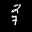
\includegraphics[scale=2]{figures/MeKKS-DIFFERENCING/frame0}
        \end{subfigure}
        \hfill
        \begin{subfigure}[t]{0.19\textwidth}
            \centering
            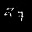
\includegraphics[scale=2]{figures/MeKKS-DIFFERENCING/frame4}
        \end{subfigure}
        \hfill
        \begin{subfigure}[t]{0.19\textwidth}
            \centering
            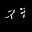
\includegraphics[scale=2]{figures/MeKKS-DIFFERENCING/frame8}
        \end{subfigure}
        \hfill
        \begin{subfigure}[t]{0.19\textwidth}
            \centering
            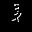
\includegraphics[scale=2]{figures/MeKKS-DIFFERENCING/frame12}
        \end{subfigure}
        \hfill
        \begin{subfigure}[t]{0.19\textwidth}
            \centering
            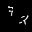
\includegraphics[scale=2]{figures/MeKKS-DIFFERENCING/frame16}
        \end{subfigure}
        \caption{Gaussian Average with MeKKS.}
    \end{subfigure}

    \caption{Moving-MNIST Inference Results}
    \label{fig:mnistInferenceResults}
\end{figure}
\setlength{\leftskip}{0cm}
\subsection{Online Mixture Model}
\setlength{\leftskip}{0.5cm}
\indent \indent
In the \textit{online mixture model} algorithm detailed in §\ref{sec:OMM}, Equation \ref{eq:gmmInequality} describes how a fitted model can be used to segment an image. However, inequality comparison operators are not provided by the standard CKKS implementation. To solve this, Cheon et al.\ proposed the algorithm in Figure \ref{fig:comparison} ~\cite{Comparison}. Unfortunately, this introduces security concerns. If the ability to compare two HE ciphertexts is added to the system, an attacker\footnote{such as Mallory in §\ref{sec:threatModel}.} could use it to exfiltrate information about the image. For example, with enough comparison operations, they would be able to determine the exact value of each pixel in a frame. Consequently, this algorithm was abandoned to preserve the security of the system.
\begin{figure}
    \centering
    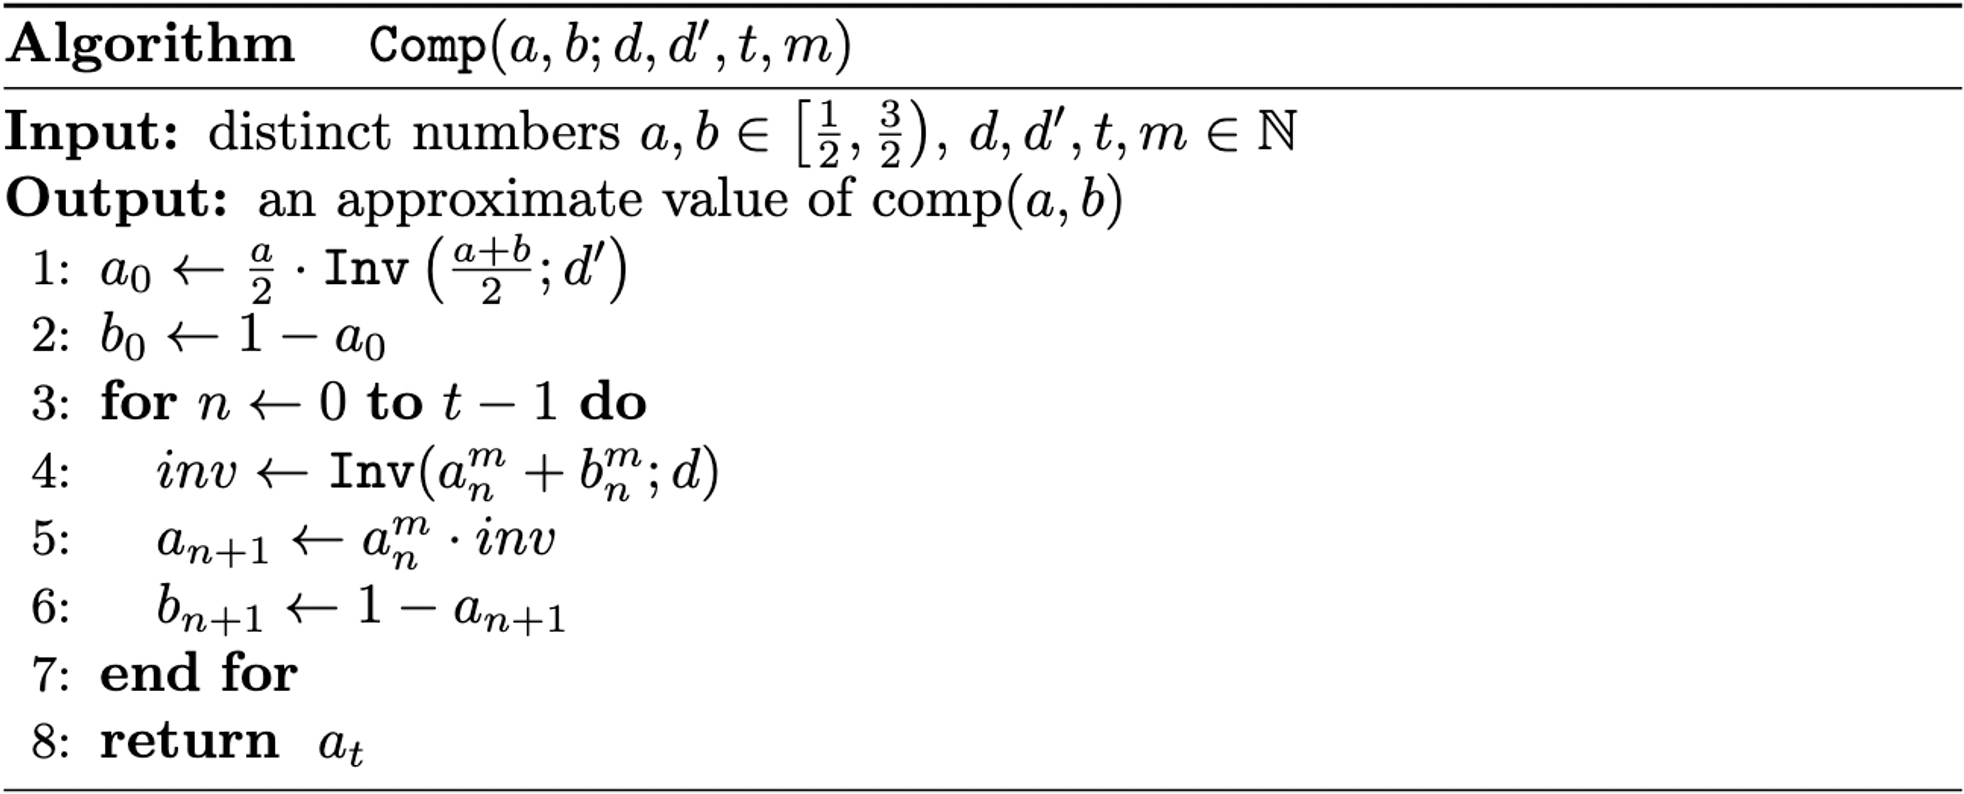
\includegraphics[width=\textwidth]{figures/algorithm1}
    \caption{Homomorphic Comparison Algorithm}
    \label{fig:comparison}
\end{figure}
\smallskip \\ \indent
For the same reason, the median filter could not be implemented. The pixel values could not be ordered without a comparison operator, so a median could not be calculated.


\setlength{\leftskip}{0cm}
\subsection{Expectation-Maximisation Algorithm}
\setlength{\leftskip}{0.5cm}
\indent \indent
The difficulty in implementing this algorithm came from the number of operations that need to be performed across the fitting and predicting stages. Calculating means and covariances repeatedly requires many successive multiplications, requiring many coefficient levels in ciphertexts. Also, like the online mixture model, not all operations are supported by the CKKS scheme. In particular, the algorithm requires several divisions to be performed when updating the Gaussian distributions. Currently, the best solution for this seems to be provided by Cheon et al.\ ~\cite{Comparison}. However, the algorithm, given in Figure \ref{fig:division}, has a minimal domain requiring input values to be between zero and two. Normalising pixel values might provide a method for incorporating this, but the noise induced by HE means inference becomes infeasibly inaccurate
\begin{figure}
    \centering
    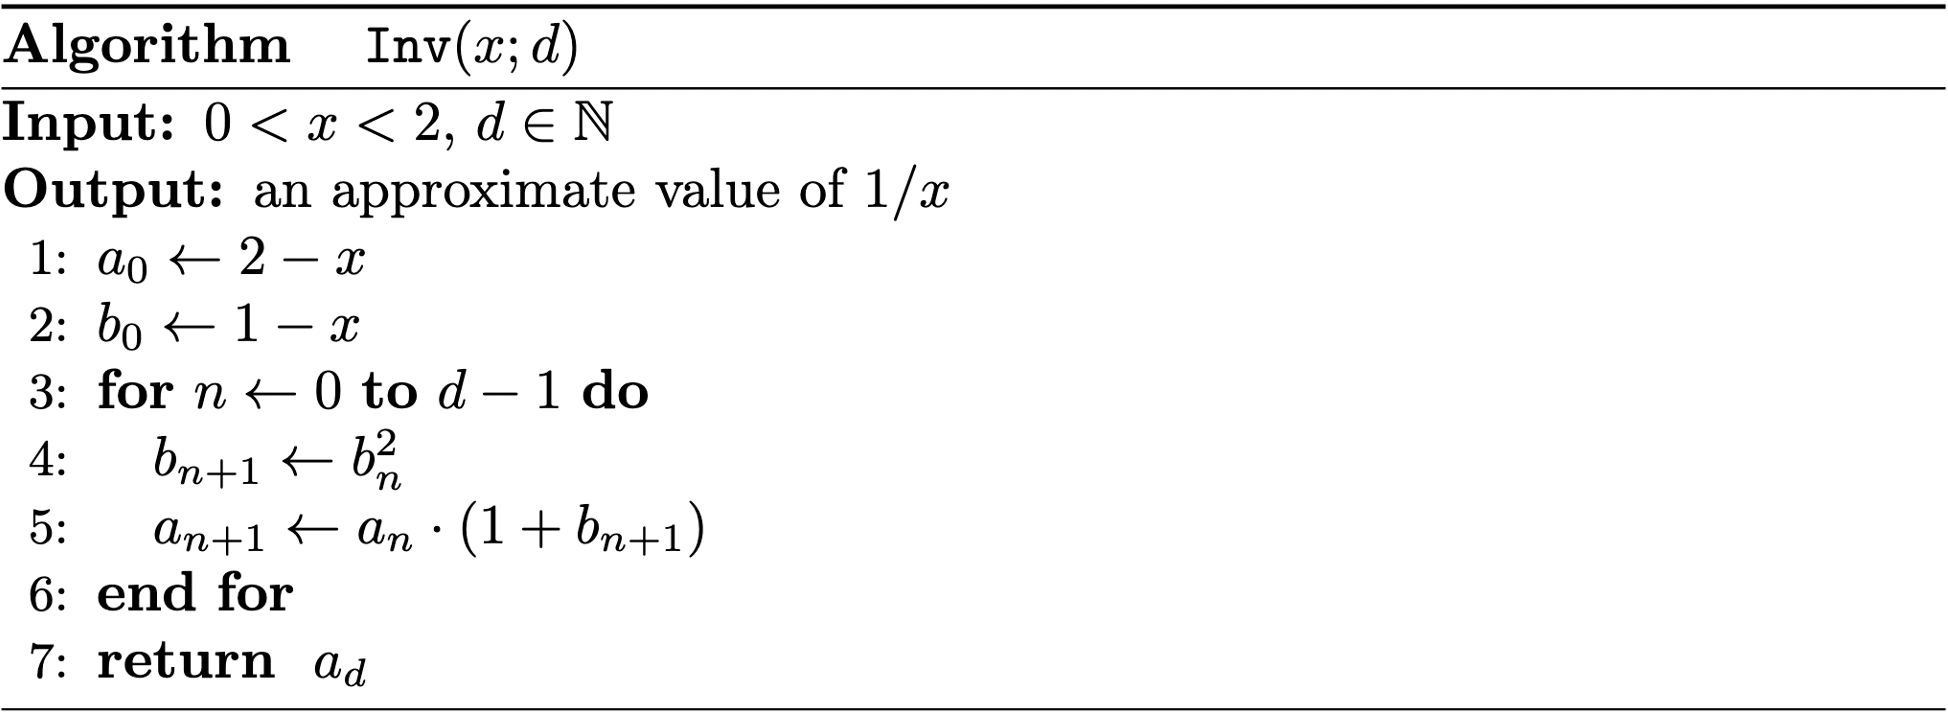
\includegraphics[width=\textwidth]{figures/algorithm2}
    \caption{Homomorphic Division Algorithm}
    \label{fig:division}
\end{figure}

\setlength{\leftskip}{0cm}




\section{Practicality}
\setlength{\leftskip}{0.25cm}
\indent \indent
This section will evaluate the implementation from the perspective of practicality in real-world surveillance systems. It will do so through two key aspects: the MLaaS client-server model and the accuracy of inference algorithms.

\setlength{\leftskip}{0cm}
\subsection{Networking}
\subsubsection{Data Handling}
\setlength{\leftskip}{0.5cm}
\indent \indent
Before data can be sent across the network, it must be \textit{packed}, and once it is received, it must be \textit{unpacked}. This proved to be a significant bottleneck before transmitting data. During the packing phase, data must be encrypted and serialised before it is transmitted over the network. To make transmission more efficient, a compression stage is added to try and reduce the memory usage of videos. Similarly, in the unpacking phase, data must be decompressed, deserialised, and decrypted to recover the video and inference results.
\smallskip \\ \indent
As described in §\ref{sec:networking}, several methods were investigated to try and reduce this bottleneck. By combining some of these techniques, substantial progress was made in reducing the time the packing and unpacking algorithms took to run. Figure \ref{fig:naivePackingAndUnpackingGraph} provides the running time of a na\"ive implementation of these algorithms, and Figure \ref{fig:packingAndUnpackingGraph} demonstrates the performance of an optimised implementation. From these charts, Table \ref{tab:packingAndUnpacking} has been derived to highlight the improvement for each category of inference and encryption scheme. Interestingly, the unpacking algorithm can be improved using parallelisation when the CKKS scheme is used, but it will worsen performance when MeKKS is used. This is due to the delays caused by deserialising data that were overcome by implementing directly in Python - although this does make the encryption and decryption functions perform dramatically worse.
\smallskip \\ \indent
While these times may appear slow, it is important to remember that surveillance companies rarely stream all video from a device. Cameras will usually contain multiple sensors to determine when the primary camera should be triggered to conserve battery life. Then, only short clips containing potential events are transferred to the server for inference. Consequently, real-time performance is not required. Although, speed cannot be ignored to ensure users are not notified too late.
\begin{figure}[h!]
    \centering
    \begin{subfigure}[b]{0.495\textwidth}
        \centering
        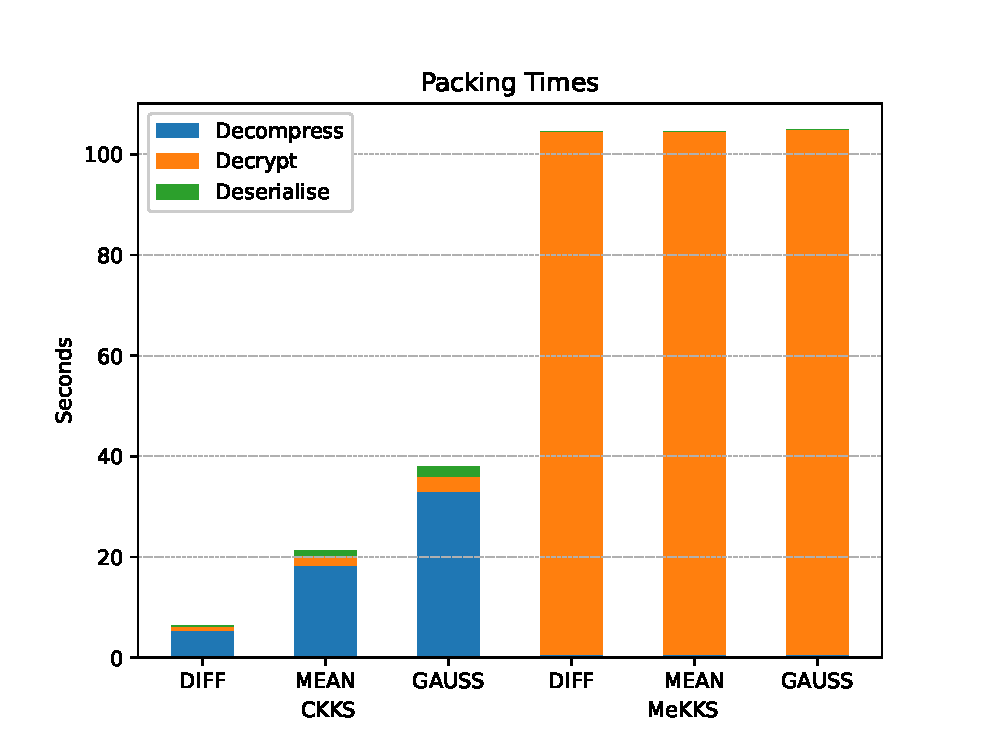
\includegraphics[width=\textwidth]{figures/naivePackingTimes}
        \caption{Packing}
    \end{subfigure}
    \hfill
    \begin{subfigure}[b]{0.495\textwidth}
        \centering
        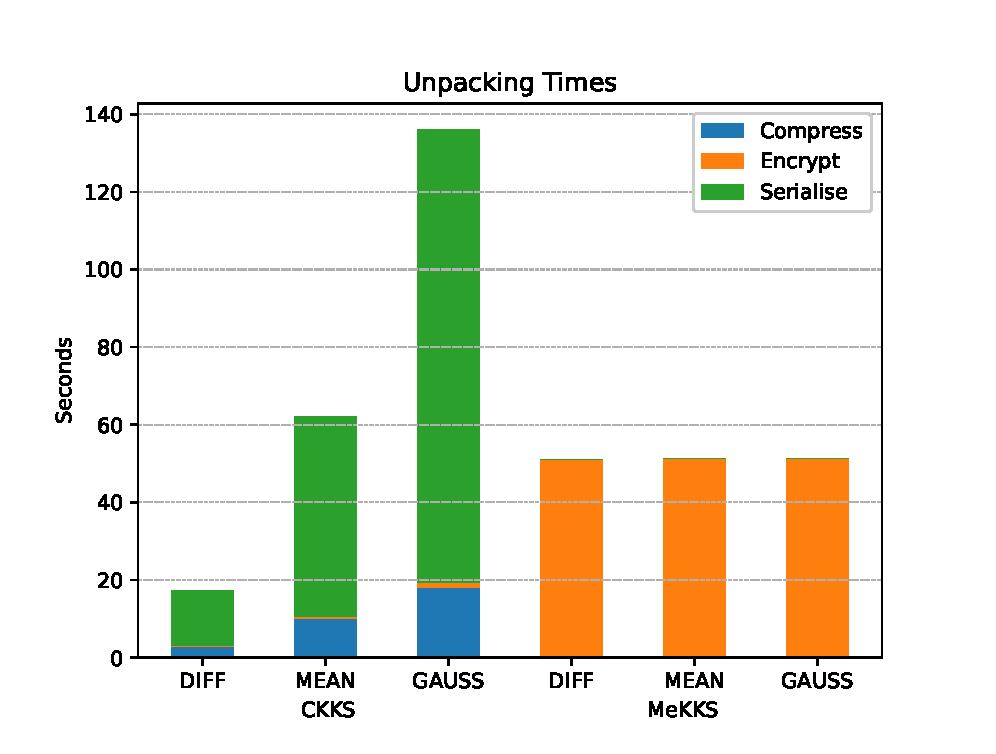
\includegraphics[width=\textwidth]{figures/naiveUnpackingTimes}
        \caption{Unpacking}
    \end{subfigure}
    \caption{Na\"ive Packing and Unpacking Times}
    \label{fig:naivePackingAndUnpackingGraph}
\end{figure}
\begin{figure}[h!]
    \centering
    \begin{subfigure}[b]{0.495\textwidth}
        \centering
        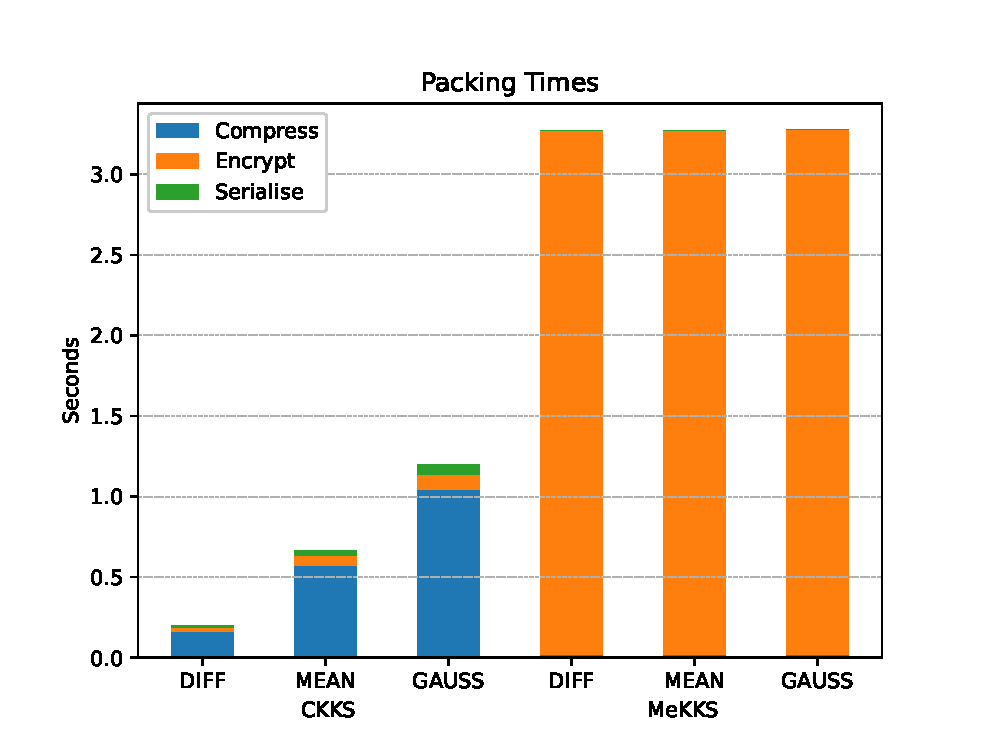
\includegraphics[width=\textwidth]{figures/packingTimes}
        \caption{Packing}
    \end{subfigure}
    \hfill
    \begin{subfigure}[b]{0.495\textwidth}
        \centering
        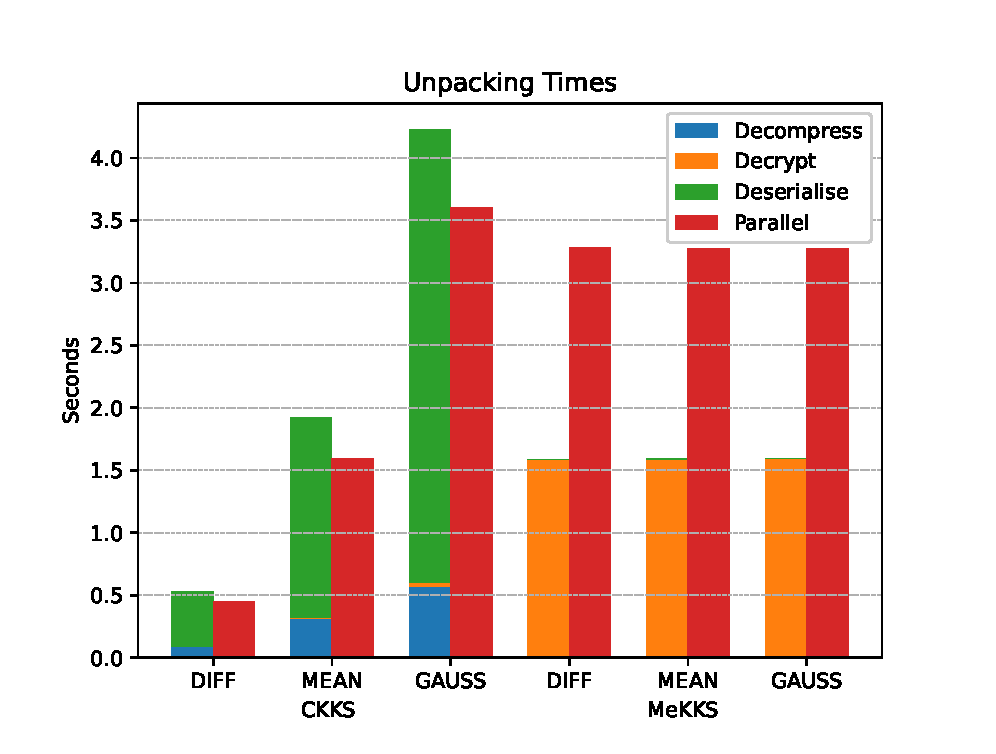
\includegraphics[width=\textwidth]{figures/unpackingTimes}
        \caption{Unpacking}
    \end{subfigure}
    \caption{Optimised Packing and Unpacking Times}
    \label{fig:packingAndUnpackingGraph}
\end{figure}
\begin{table}[h!]
    \centering
    \def\arraystretch{1.25}
    \resizebox{\textwidth}{!}{%
    \begin{tabular}{|c|c|c|c|c|c|}
        \hline
        \textrm{\textbf{Encryption}} & \textrm{\textbf{Inference}} & \textrm{\textbf{Process}} & \textrm{\textbf{Na\"ive} (s)} & \textrm{\textbf{Optimised} (s)} & \textrm{\textbf{Improvement}}
        \\ \hline \hline
        \multirow{6}{*}{\textrm{CKKS}}  & \multirow{2}{*}{\textrm{Differencing}} & \textrm{Packing}   & $6.440$ & $0.198$ & $32.5 \times$
        \\ \cline{3-6} 
                                        &                                        & \textrm{Unpacking} & $17.349$ & $0.850$ & $20.4 \times$
        \\ \cline{2-6} 
                                        & \multirow{2}{*}{\textrm{Mean}}         & \textrm{Packing}   & $21.376$ & $0.668$ & $32.0 \times$
        \\ \cline{3-6} 
                                        &                                        & \textrm{Unpacking} & $62.058$ & $3.095$ & $20.1 \times$
        \\ \cline{2-6} 
                                        & \multirow{2}{*}{\textrm{Gaussian}}     & \textrm{Packing}   & $38.003$ & $1.200$ & $31.7 \times$
        \\ \cline{3-6} 
                                        &                                        & \textrm{Unpacking} & $136.008$ & $7.108$ & $19.1 \times$
        \\ \hline
        \multirow{6}{*}{\textrm{MeKKS}} & \multirow{2}{*}{\textrm{Differencing}} & \textrm{Packing}   & $104.529$ & $3.273$ & $31.9 \times$
        \\ \cline{3-6} 
                                        &                                        & \textrm{Unpacking} & $51.076$ & $1.589$ & $32.1 \times$
        \\ \cline{2-6} 
                                        & \multirow{2}{*}{\textrm{Mean}}         & \textrm{Packing}   & $104.604$ & $3.274$ & $31.9 \times$
        \\ \cline{3-6} 
                                        &                                        & \textrm{Unpacking} & $51.202$ & $1.590$ & $32.2 \times$
        \\ \cline{2-6} 
                                        & \multirow{2}{*}{\textrm{Gaussian}}     & \textrm{Packing}   & $104.884$ & $3.277$ & $32.0 \times$
        \\ \cline{3-6} 
                                        &                                        & \textrm{Unpacking} & $51.319$ & $1.596$ & $32.2 \times$
        \\ \hline
    \end{tabular}
    }
    \caption[Packing and Unpacking Improvements]{Packing and unpacking times for each encryption scheme and inference algorithm, and the improvement gained.}
    \label{tab:packingAndUnpacking}
\end{table}

\setlength{\leftskip}{0cm}
\subsubsection{Transmission Times}
\setlength{\leftskip}{0.5cm}
\indent \indent
The other key aspect of the network component of the project is transmitting the data. One fundamental flaw of HE is the memory consumption inflation caused by encrypting data. Consequently, transmission times are much slower than when working with plain video data. In the final application, two main techniques were used to reduce this impact: vectorisation and compression.
\smallskip \\ \indent
For compression, several algorithms were tested - they were compared for both running time and compression ratio - and the algorithm that performed best on CKKS data was selected. The results of these tests are included in Table \ref{tab:compression}. From this, the impact of compressing videos is shown in Figure \ref{fig:compression1}. MeKKS's more basic implementation means the ciphertext size is constant for all inference methods. Despite this, it is still two orders of magnitude smaller than CKKS data, thanks to the native Python data structures used. Compression is much more significant with CKKS data, almost halving the memory usage for the Gaussian inference, making it a valuable component of the CKKS packing procedure, but largely unnecessary when MeKKS is selected.
\smallskip \\ \indent
Already, this provides good improvements over raw data. However, this can be extended by encrypting rows of video frames as a single ciphertext rather than each pixel distinctly. Figure \ref{fig:compression2} depicts the results of this adaptation.
\smallskip \\ \indent
As a result of the above optimisations, the running times for the client and server are summarised by Figure \ref{fig:clientTimeGraph} and Figure \ref{fig:serverTimeGraph} respectively.
\begin{table}
    \centering
    \def\arraystretch{1.25}
    % \resizebox{\textwidth}{!}{%
    \begin{tabular}{|c||c|c|c|c|}
        \hline
        \textrm{\textbf{Algorithm}} & \textrm{\textbf{Compression} (s)} & \textrm{\textbf{Decompression} (s)} & \textrm{\textbf{Size} (KB)} & \textrm{\textbf{Percentage}}
        \\ \hline \hline
        \textrm{None} & - & - & $716.18$ & $100\%$
        \\ \hline
        \texttt{gzip} & $94.69$ & $3.55$ & $442.46$ & $61.78\%$
        \\ \hline
        \texttt{bz2} & $36.28$ & $5.02$ & $435.29$ & $60.78\%$
        \\ \hline
        \texttt{lzma} & $294.85$ & $20.98$ & $421.86$ & $58.9\%$
        \\ \hline
        \texttt{brotli} & $871.97$ & $0$ & $435.78$  & $60.85\%$
        \\ \hline
    \end{tabular}
    % }
    \caption[Compression algorithms]{Evaluation of compression algorithms.}
    \label{tab:compression}
\end{table}
\begin{figure}[h!]
    \centering
    \begin{subfigure}[b]{0.495\textwidth}
        \centering
        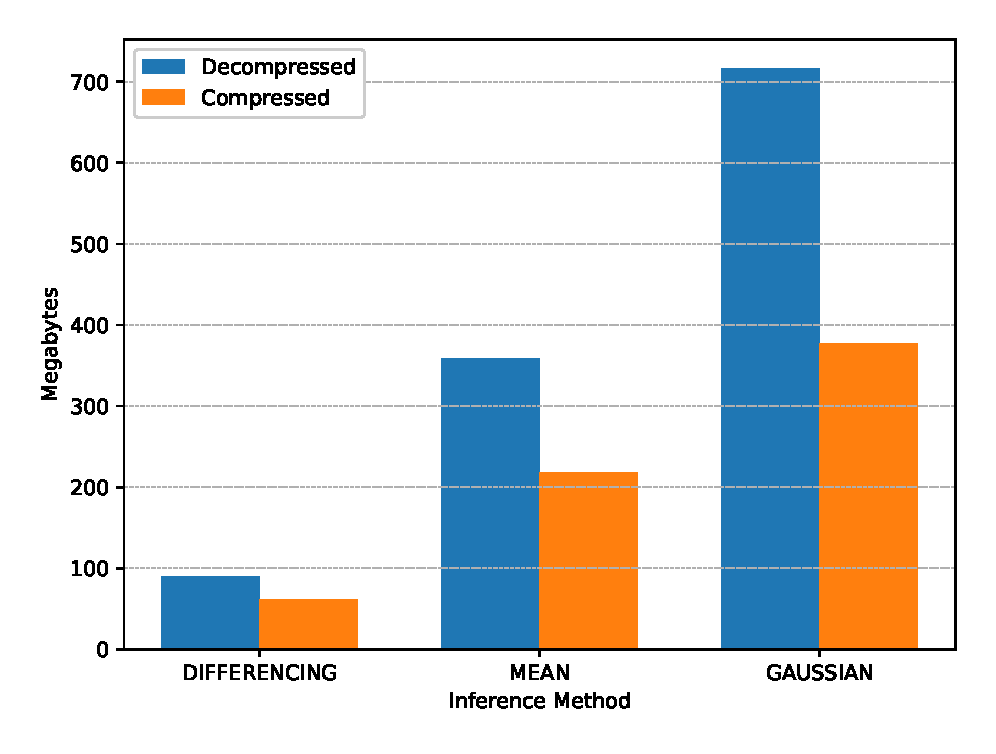
\includegraphics[width=\textwidth]{figures/naiveMemUsageCKKS}
        \caption{CKKS}
    \end{subfigure}
    \hfill
    \begin{subfigure}[b]{0.495\textwidth}
        \centering
        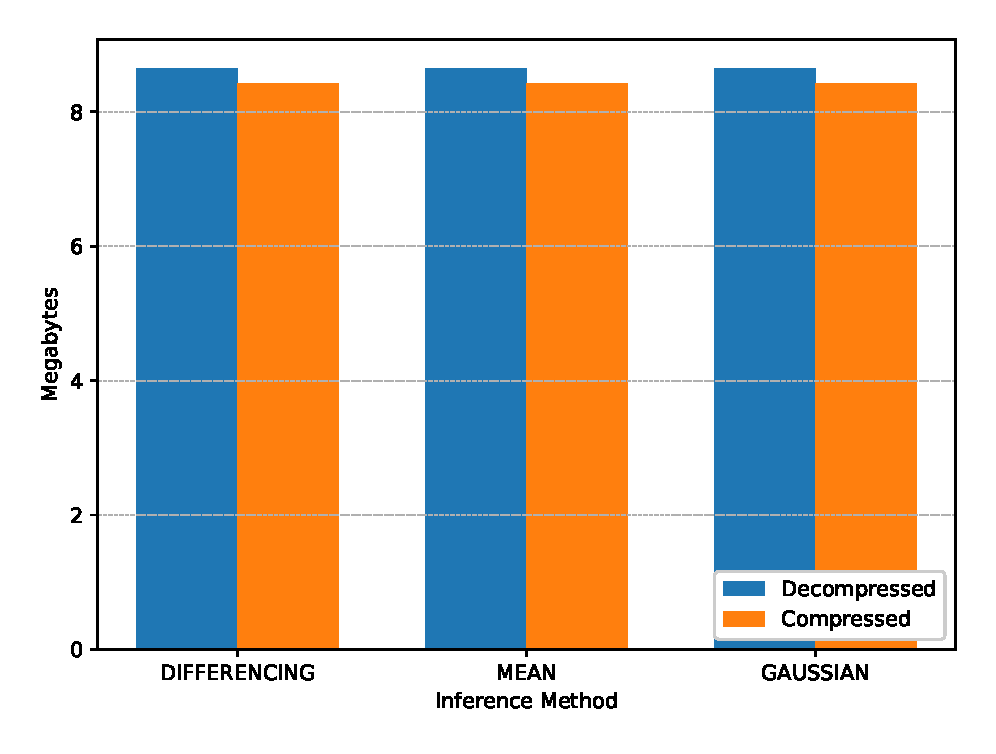
\includegraphics[width=\textwidth]{figures/naiveMemUsageMeKKS}
        \caption{MeKKS}
    \end{subfigure}
    \caption{Na\"ive Memory Usage Compression Comparison}
    \label{fig:compression1}
\end{figure}
\begin{figure}[h!]
    \centering
    \begin{subfigure}[b]{0.495\textwidth}
        \centering
        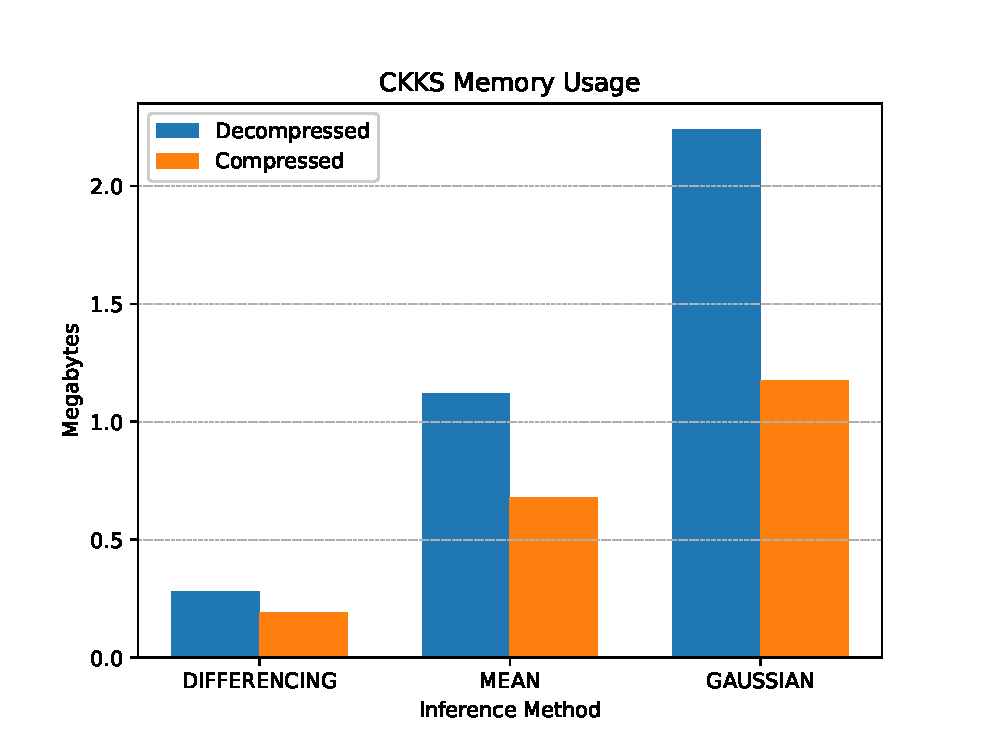
\includegraphics[width=\textwidth]{figures/memUsageCKKS}
        \caption{CKKS}
    \end{subfigure}
    \hfill
    \begin{subfigure}[b]{0.495\textwidth}
        \centering
        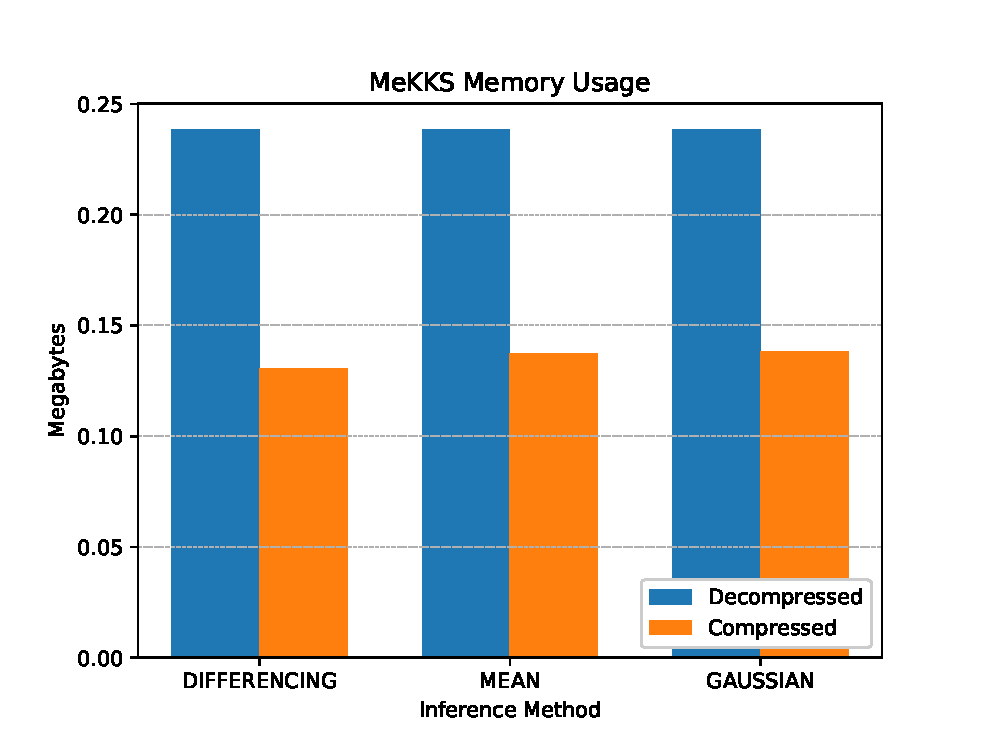
\includegraphics[width=\textwidth]{figures/memUsageMeKKS}
        \caption{MeKKS}
    \end{subfigure}
    \caption{Vectorised Memory Usage Compression Comparison}
    \label{fig:compression2}
\end{figure}
\begin{figure}[h!]
    \centering
    \begin{subfigure}[t]{0.495\textwidth}
        \centering
        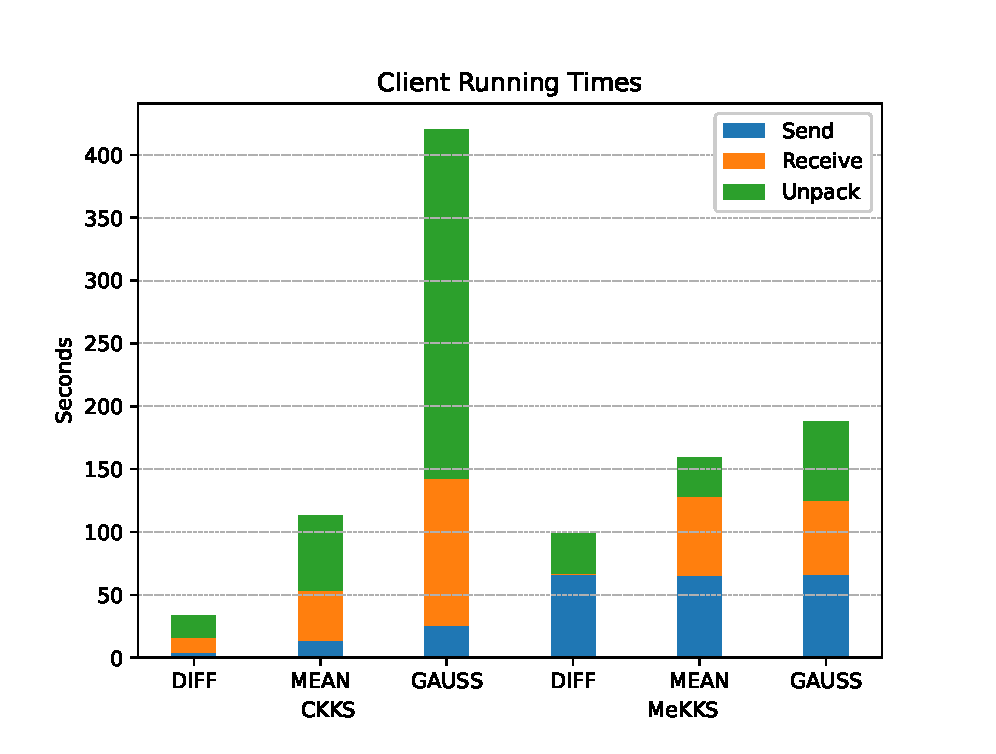
\includegraphics[width=\textwidth]{figures/clientTimes}
        \caption{Client Running Times}
        \label{fig:clientTimeGraph}
    \end{subfigure}
    \hfill
    \begin{subfigure}[t]{0.495\textwidth}
        \centering
        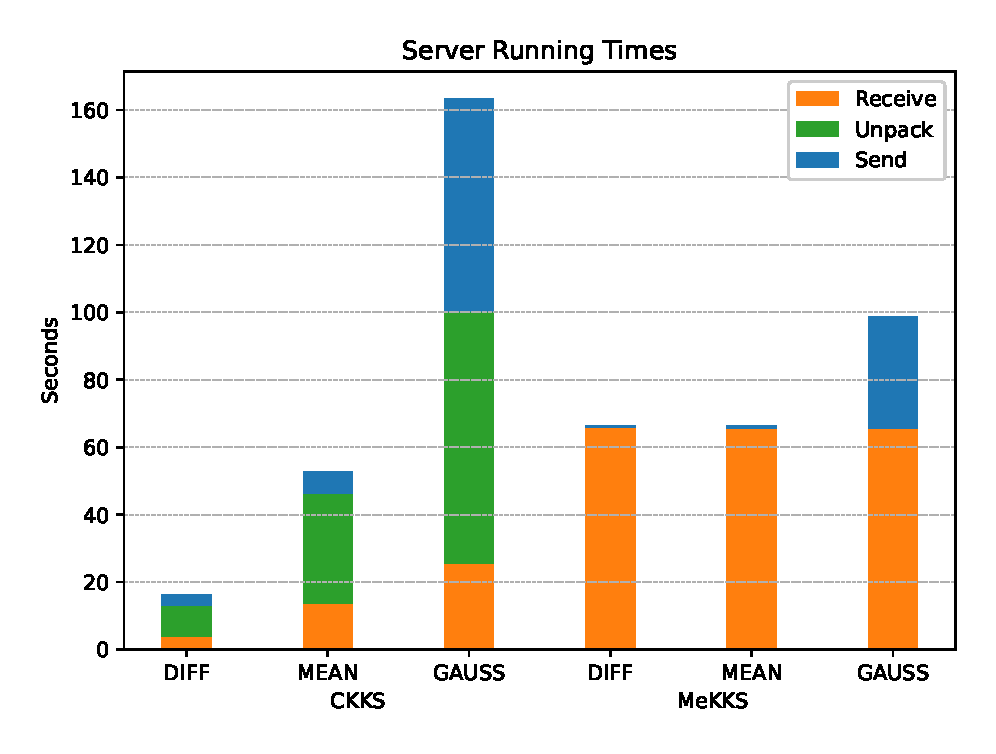
\includegraphics[width=\textwidth]{figures/serverTimes}
        \caption{Server Running Times}
        \label{fig:serverTimeGraph}
    \end{subfigure}
    \caption{Client and Server Running Times}
    \label{fig:clientAndServerGraph}
\end{figure}

\setlength{\leftskip}{0cm}

\subsection{Inference}
\setlength{\leftskip}{0.5cm}
\indent \indent
Another area of investigation that must be considered when discussing practicality is the performance of inference algorithms. This can be approached from two metrics. Firstly, the \textit{running time} must be considered to evaluate if algorithms will be able to return results in a reasonable amount of time. Secondly, \textit{accuracy} must be analysed to assess the quality of inference results compared to plain inference.

\setlength{\leftskip}{0cm}
\subsubsection{Running Time}
\setlength{\leftskip}{0.5cm}
\indent \indent
The running time for each inference algorithm varies significantly and is severely impacted by the parameters used to tune the accuracy of each algorithm, as discussed in §\ref{sec:adaptations}. Therefore, for this comparison, the parameters were tuned using the CKKS scheme and kept constant for a fair evaluation when testing the MeKKS scheme. The results are depicted by Figure \ref{fig:inferenceTime}. As expected, the CKKS scheme runs much quicker than the MeKKS scheme due to the more optimised implementation.

\begin{figure}[h!]
    \centering
    \begin{subfigure}[b]{0.495\textwidth}
        \centering
        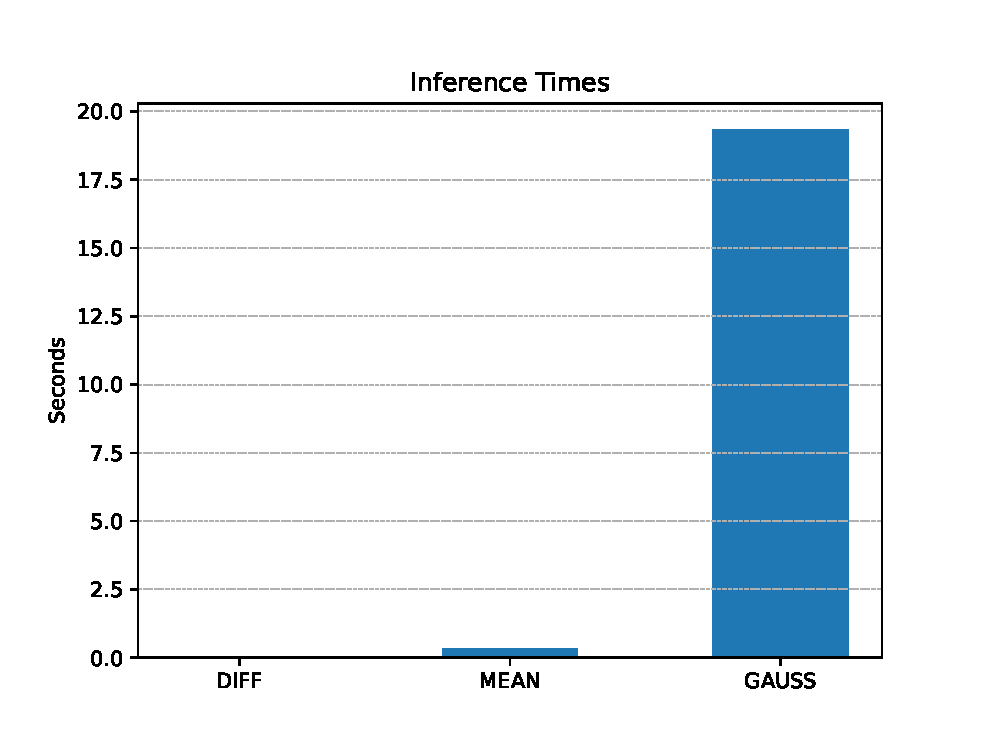
\includegraphics[width=\textwidth]{figures/inferenceTimesCKKS}
        \caption{CKKS}
    \end{subfigure}
    \hfill
    \begin{subfigure}[b]{0.495\textwidth}
        \centering
        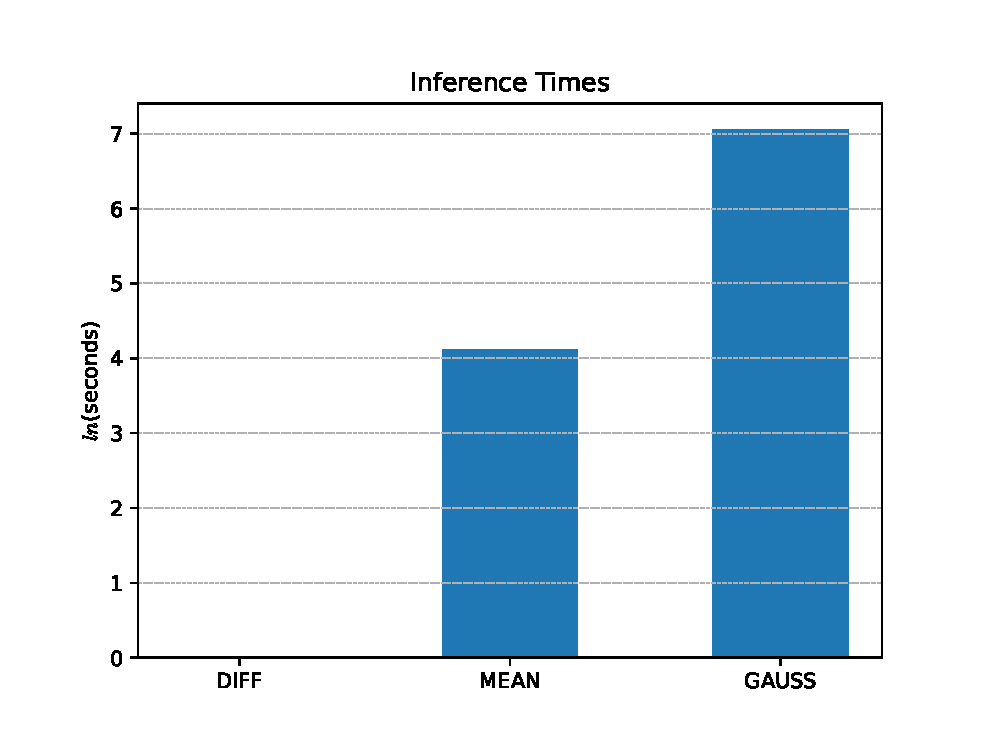
\includegraphics[width=\textwidth]{figures/inferenceTimesMeKKS}
        \caption{MeKKS}
    \end{subfigure}
    \caption{Inference Times}
    \label{fig:inferenceTime}
\end{figure}

\setlength{\leftskip}{0cm}
\subsubsection{Accuracy}
\setlength{\leftskip}{0.5cm}
\indent \indent
The accuracies of each HE inference algorithm are compared in Figure \ref{fig:accuracy}. While the HE implementations do not exactly match inference in unencrypted data, they are able to produce nearly the same accuracy, producing almost identical results to the human eye. Perhaps surprisingly, MeKKS produces slightly more accurate results with frame differencing, but this is likely due to the random noise induced by HE encryption.  
\smallskip \\ \indent
The Moving-MNIST dataset allows accuracy to be easily calculated because it only contains white moving objects on a black background. Therefore, the similarity between the inference result and the original video can be determined by calculating the \textit{sum square difference} according to Equation \ref{eq:sumSquareDiff}

\begin{equation}
    \label{eq:sumSquareDiff}
    \begin{split}
    &S_{sq} = \sum_{n,m \in N^{N \times M}} (J[n, m] - I[n, m])^2 \\
    &\textrm{which can be normalised using} \\
    &\frac{S_{sq}}{\sqrt{\sum J[n,m]^2 \times \sum I[n,m]^2}}
    \end{split}
\end{equation}
given two images $J[x,y]$ and $I[x,y]$ with $(x,y) \in N^{N \times M}$.
\begin{figure}[h!]
    \centering
    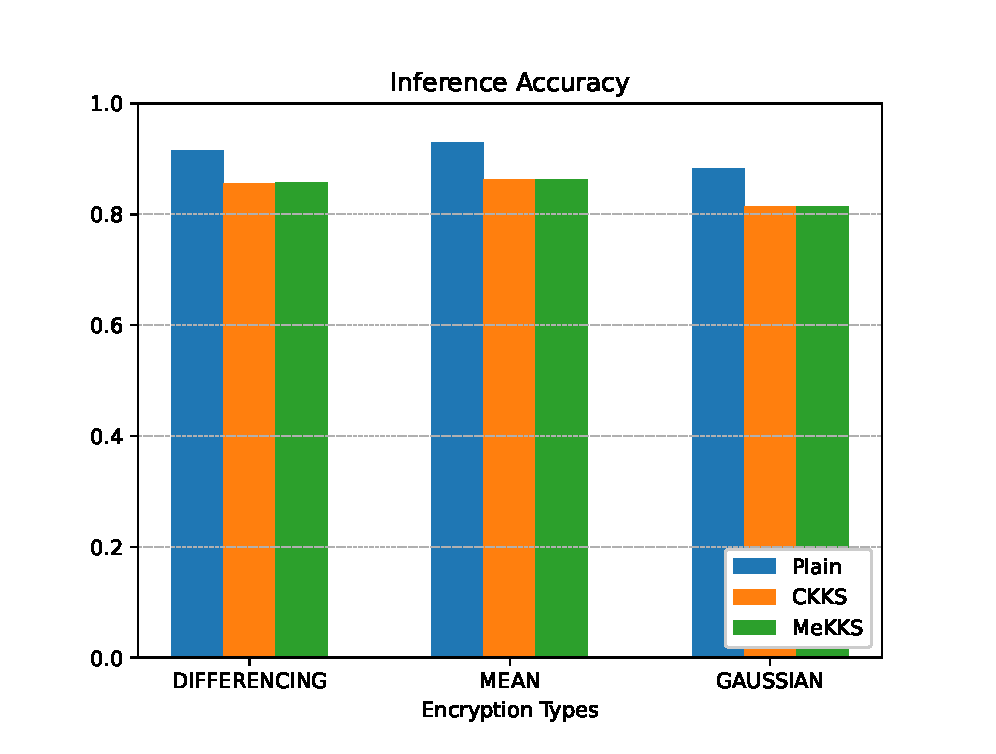
\includegraphics[scale=0.6]{figures/accuracy}
    \caption{Inference Accuracy}
    \label{fig:accuracy}
\end{figure}

\setlength{\leftskip}{0cm}
\subsubsection{Energy Usage}
\setlength{\leftskip}{0.5cm}
\indent \indent
While not a particular focus of this investigation, energy usage is an important factor in determining the practicality of HE in surveillance. This is because the majority of devices being emulated - surveillance cameras or doorbells - are battery-powered. As such, they must be conservative in their energy usage in order to extend battery life as far as possible. Figure \ref{fig:energy} depicts the energy usage of each combination of encryption scheme and inference method for the client and server modules. The absolute value cannot be isolated from background energy usage, so values have been normalised to allow for comparison on a log scale.
\begin{figure}[h!]
    \centering
    \includegraphics[scale=0.6]{figures/energyUsage}
    \caption{Energy Usage}
    \label{fig:energy}
\end{figure}

\setlength{\leftskip}{0cm}




\section{Summary}
\setlength{\leftskip}{0.25cm}
\indent \indent
This evaluation provides evidence that combining the domains of homomorphic encryption and moving object detection can produce promising results comparable to existing algorithms extracting moving objects from unencrypted, plain video data. Moreover, it demonstrates that progress can be made in improving the performance of systems incorporating these techniques. However, it acknowledges that further research is required into homomorphic primitives to provide more operations on encrypted data and reduce the space complexity of encrypted data to improve the time complexity of data transmission and inference algorithms.

\setlength{\leftskip}{0cm}
